\documentclass[a4paper]{scrartcl}
\usepackage[cm]{fullpage}
\usepackage{amsmath, amssymb, esint}
\usepackage{siunitx}
\usepackage{listings}
\usepackage[backend = biber, style = numeric-comp]{biblatex}

\usepackage{tikz, pgfplots}
\pgfplotsset{
    compat = 1.9,
    plot/.style = {
        axis lines = middle,
        clip = false
    },
    plot-scatter/.style = {
        only marks
    }
}

\begin{filecontents}{\jobname.bib}
@misc{BGI2016,
    url = {http://bgi.omp.obs-mip.fr/data-products/Toolbox/Prediction-of-gravity-value},
    year  = {2016},
    month = {apr},
    title = {Prediction of gravity value},
    author = {The International Gravimetric Bureau ({BGI})},
    howpublished = {Online tool}
}
\end{filecontents}
\addbibresource{\jobname.bib}

\begin{document}

\title{PHYS2113: Coupled Pendula}
\author{ \\ \\ }
\date{2016-04-20}
\maketitle

\section{Introduction}
Please refer to the student notes of the experiment.

\section{Materials and Methods}
Please refer to the operating instructions and prework of the experiment.

Local gravity was assumed to be \(g = \SI{9.797}{\metre\per\second\squared}\) \cite{BGI2016} at the second year lab (\SI{33.918}{\degree}S \SI{151.2303}{\degree}E) at an estimated altitude of \SI{50}{\metre}.

The displacement value (\(\Delta x\)) recorded while measuring the spring's spring constant was zeroed at the first mass, to avoid the typical initial non-linearity of a spring under very little tension.

The Hamming windowed DFT was used to determine the frequencies since it is a low-leakage narrowband window, except when the couple length was \(l = \SI{20}{\centi\metre}\) where the DFT was unwindowed, since the frequencies were too close together for any other window. The uncertainty in frequency was defined to be where the power falls below \SI{-20}{\deci\bel} of the peak bin. This was done visually after having \emph{Mathematica} graph the frequency data, with template code in Listing \ref{lst:analysis}.

The pendula was started with initial angle less than \(\frac{\pi}{10} \:\SI{}{\radian}\) in either direction, to allow the \(\cos \phi \approx 1\) approximation to hold, and data collected for about 4 minutes each.

\begin{lstlisting}[
    caption = \emph{Mathematica 10.2} source used to compute the DFT,
    label = lst:analysis,
    language = Mathematica,
    frame = single,
    basicstyle = \tiny
]
sampleRate = 200;
addTime[list_] := MapIndexed[{N[(#2[[1]] - 1) / sampleRate], #1} &, list];
window[list_, windowFunc_] := MapIndexed[windowFunc[(#2[[1]] - 1) / (Length[list] - 1) - 0.5] #1 &, list];
relPowerFourier[list_, windowFunc_] := MapIndexed[
    {N[(#2[[1]] - 1) sampleRate / Length[list]], #1} &,
    Take[
        20 Log10@(#1 / Max[#1] &)@Abs@Fourier[window[list, windowFunc], FourierParameters -> {1, -1}],
        Ceiling[Length[list] / 2]
    ] /. Indeterminate -> -Infinity
];
relPowerFourier[list_] := relPowerFourier[list, HammingWindow];
import[filename_] := Transpose[{#1[[2]], #1[[4]]} & /@ Drop[Import[filename], 3]];

data = Drop[#1, 40 sampleRate] & /@ import["93cm-1-extra-separation.tsv"];
fourierData = ParallelMap[relPowerFourier[#1] &, data];
ListPlot[
    fourierData, PlotRange -> {{0, 2}, {-80, 0}},
    Joined -> True, PlotMarkers -> None, ImageSize -> 700,
    PlotLegends -> Placed[{"Pendulum 1", "Pendulum 2"}, Above],
    AxesLabel -> {"Frequency (Hz)", "Relative Power (dB)"}
]
\end{lstlisting}

\section{Results}
\begin{figure}
    \centering
    \begin{tikzpicture}
        \begin{axis}[
            plot,
            xlabel = \(\Delta x\) (\si{\centi\metre}),
            ylabel = \(m\) (\si{\gram}),
            xmin = 0,
            ymin = 0
        ]
            \addplot +[plot-scatter] table [x = Delta-x, y = m, col sep = tab] {spring.tsv};
            \addplot +[no marks, domain = 0:13] {10.1655 + 3.17079 * x};
        \end{axis}
    \end{tikzpicture}
    \caption{Data from measuring the spring constant}
    \label{fig:spring}
\end{figure}

\begin{figure}
    \centering
    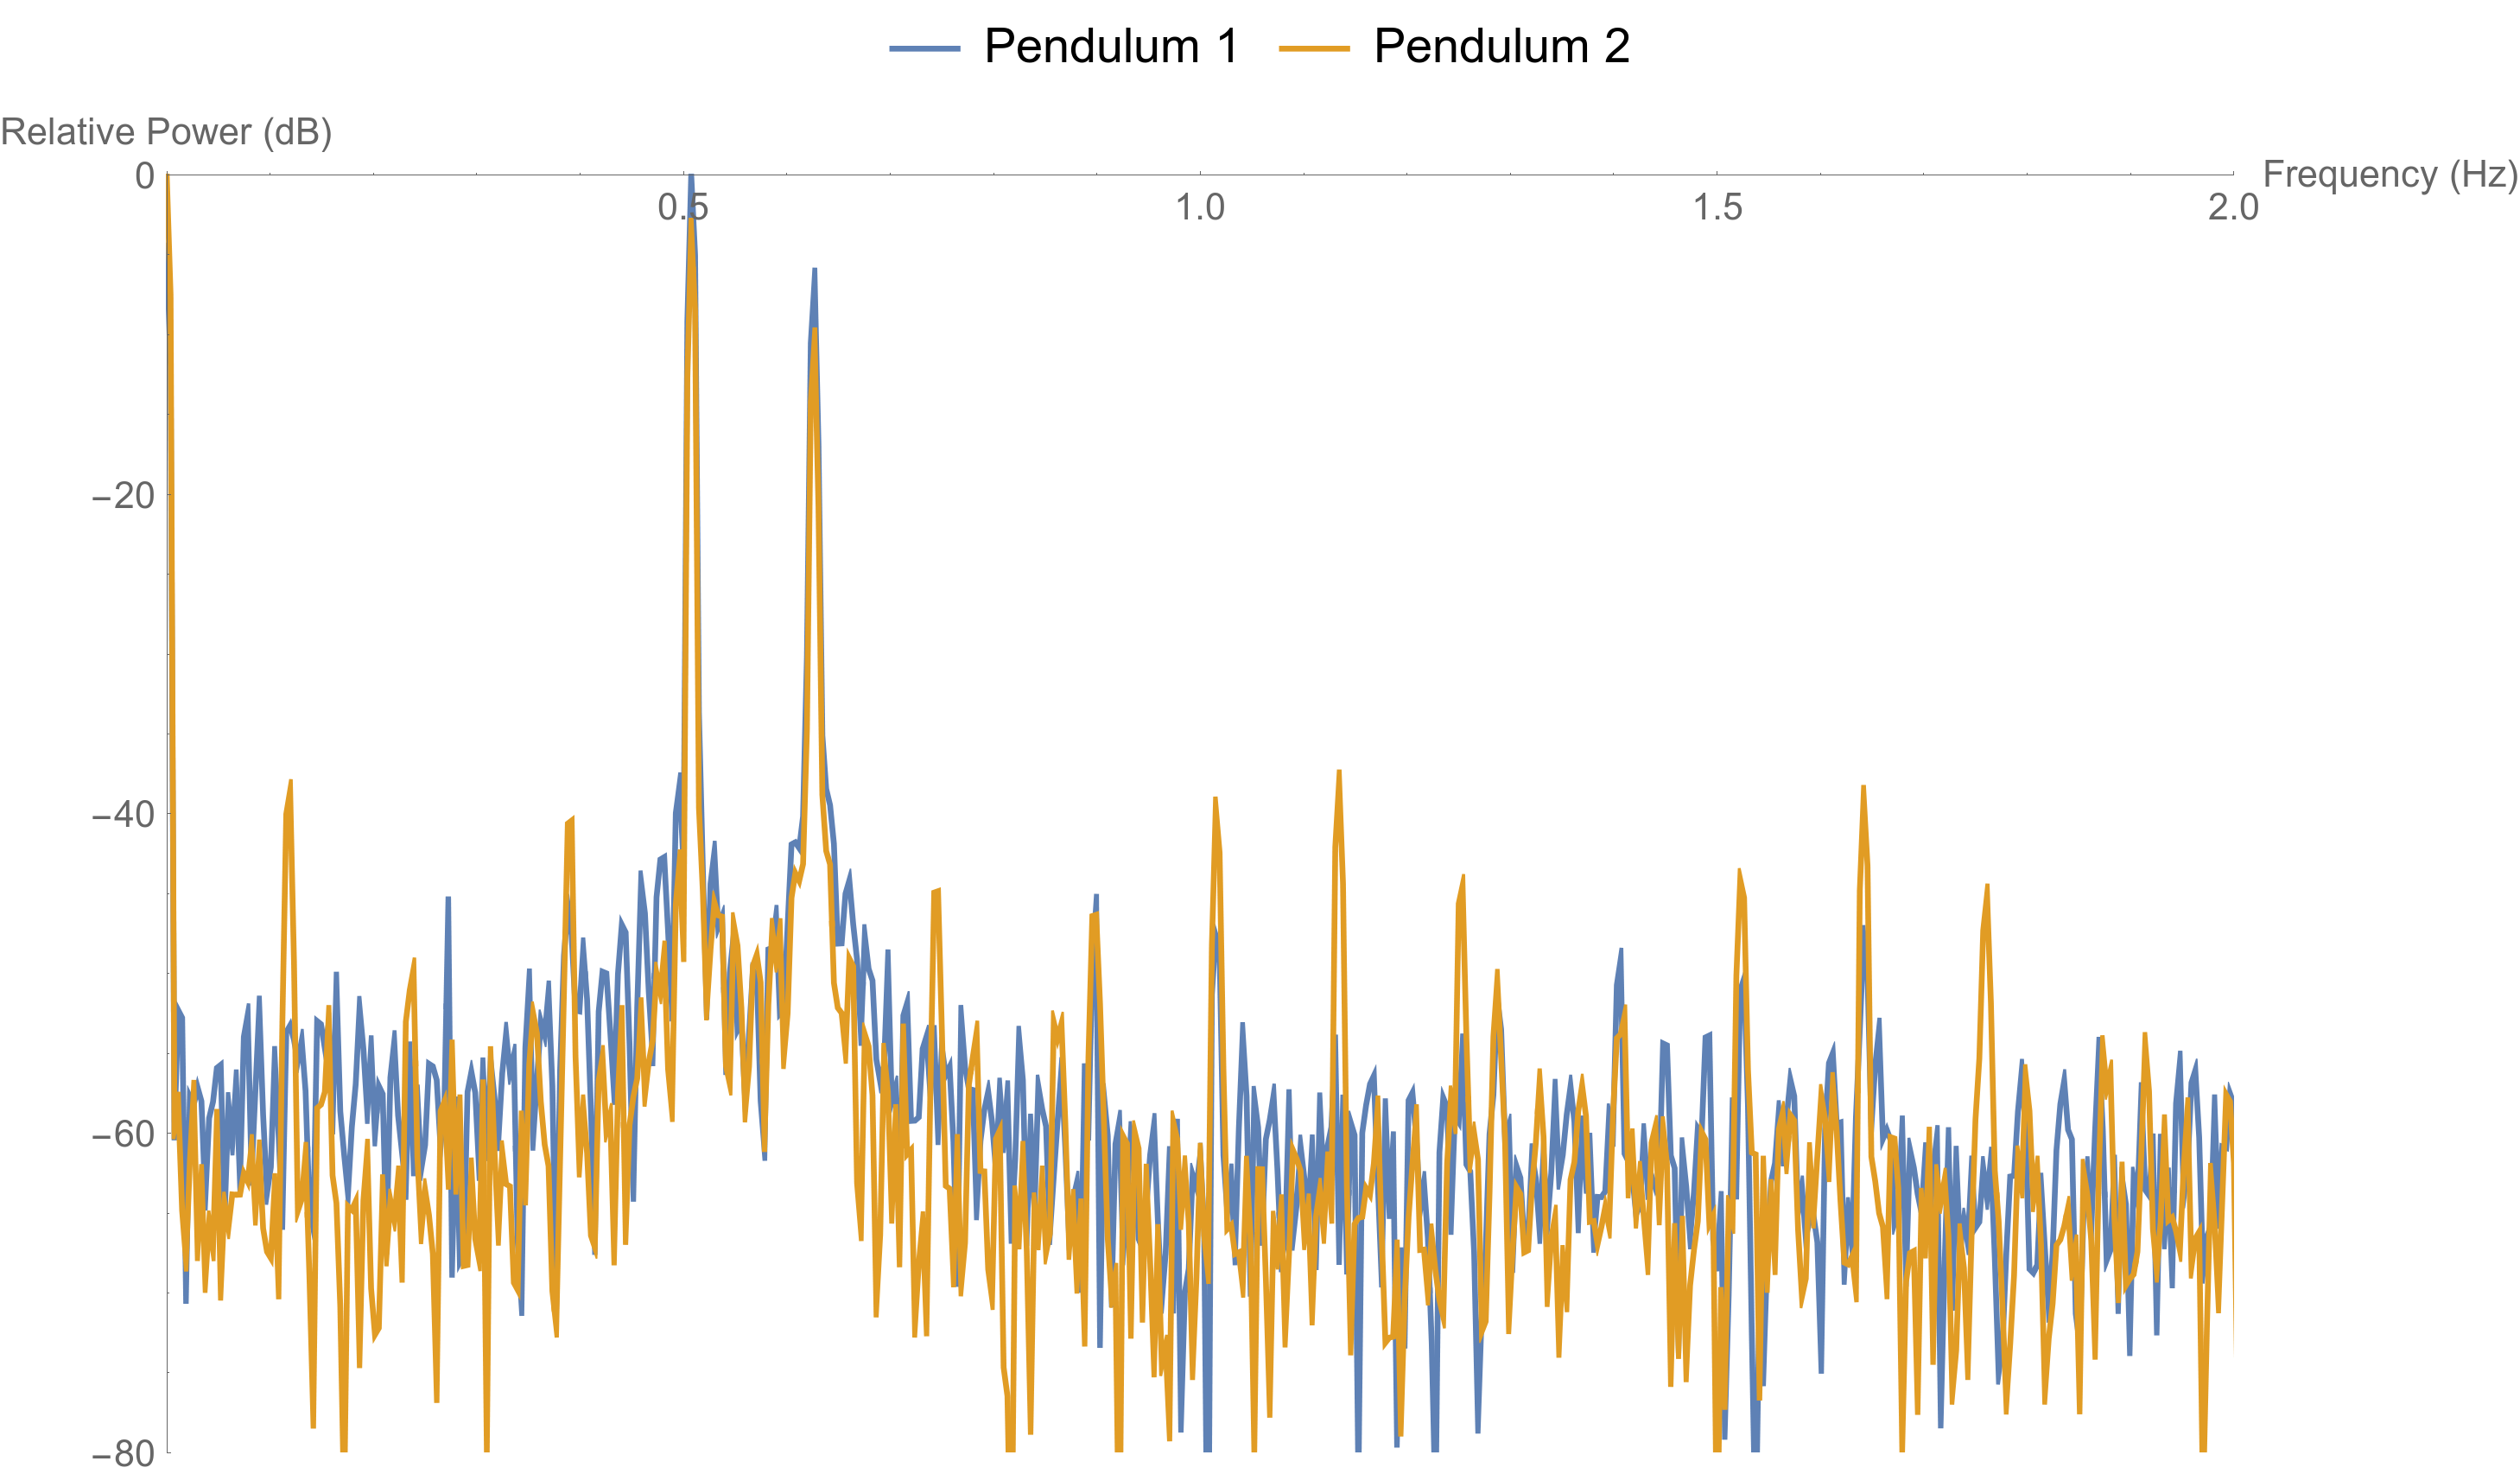
\includegraphics[width = 18cm]{93cm-1-extra-separation.png}
    \caption{Frequency analysis of beating oscillation mode at \SI{93}{\centi\metre} coupling length}
    \label{fig:example}
\end{figure}

\begin{table}
    \centering
    \begin{tabular}{c | c | c | c | c}
        Couple Length \(l\) (\si{\centi\metre}) & P1 \(f_1\) (\si{\milli\hertz}) & P2 \(f_1\) (\si{\milli\hertz}) & P1 \(f_2\) (\si{\milli\hertz}) & P2 \(f_2\) (\si{\milli\hertz}) \\
        \hline
        Uncoupled & N/A & N/A & \SI{507 \pm 6}{} & \SI{507 \pm 7}{} \\
        \SI{20.0 \pm 0.2} & \SI{513 \pm 7}{} & \SI{513 \pm 7}{} & \SI{507 \pm 7}{} & \SI{507 \pm 7}{} \\
        \SI{40.0 \pm 0.2} & \SI{528 \pm 6}{} & \SI{529 \pm 6}{} & \SI{508 \pm 8}{} & \SI{507 \pm 5}{} \\
        \SI{60.0 \pm 0.2} & \SI{551 \pm 7}{} & \SI{551 \pm 7}{} & \SI{507 \pm 5}{} & \SI{507 \pm 5}{} \\
        \SI{93.0 \pm 0.2} & \SI{627 \pm 5}{} & \SI{627 \pm 5}{} & \SI{507 \pm 6}{} & \SI{507 \pm 6}{} \\
    \end{tabular}
    \caption{Measured pendulum oscillation frequencies. P\(n\) = Pendulum \(n\)}
    \label{tab:pendula}
\end{table}

The bobs on the pendula were measured to have mass \(m = \SI{1.02 \pm 0.005}{\kilo\gram}\) and radius \SI{4.0 \pm 0.05}{\centi\metre} each. The length of the pendula from axle to centre-of-bob was \(L = \SI{97.6 \pm 0.05}{\centi\metre}\). The pendula's rods was unable to be removed from the assembly to measure its mass, but appeared to be a lightweight hollow metal tube.

Measurement of the spring's spring constant (Figure \ref{fig:spring}) produced a gradient of \SI{3.171}{\gram\per\centi\metre} with a standard error of \SI{0.011}{\gram\per\centi\metre} using \emph{Mathematica 10.2}'s \texttt{LinearModelFit[]} function under the default options, corresponding to a spring constant of \(k = \SI{3.106 \pm 0.022}{\newton\per\metre}\).

The spring was observed to be fairly ``loose'' hanging when coupled to the pendula, with a noticeable amount of sag. At equilibrium, the pendula were observed to be parallel, however.

Frequency analysis of the pendulum oscillations produced the data in Table \ref{tab:pendula}. The same frequencies were produced regardless of the oscillation mode, but the in phase mode only produced the \(f_2\) frequency, while out of phase only produced the \(f_1\). When uncoupled, the pendula only produced the \(f_2\) frequency.

A representative example of the frequency analysis can be seen in Figure \ref{fig:example}. Other than the two main peaks already described above, there are many smaller peaks (ignoring the DC offset) scattered about, some of which are harmonics of the main two peaks. The other peaks seem to be harmonics of two fundamental modes at around \SI{117 \pm 10}{\milli\hertz} and \SI{154 \pm 15}{\milli\hertz}.

\section{Discussion}
\begin{table}
    \centering
    \begin{tabular}{c | c | c}
        Couple Length \(l\) (\si{\centi\metre}) & \(f_1\) (\si{\milli\hertz}) & \(f_2\) (\si{\milli\hertz}) \\
        \hline
        Uncoupled & N/A & \SI{504.2 \pm 0.1}{} \\
        \SI{20.0 \pm 0.2} & \SI{510.6 \pm 0.2}{} & \SI{504.2 \pm 0.1}{} \\
        \SI{40.0 \pm 0.2} & \SI{529.3 \pm 0.4}{} & \SI{504.2 \pm 0.1}{} \\
        \SI{60.0 \pm 0.2} & \SI{559.1 \pm 0.6}{} & \SI{504.2 \pm 0.1}{} \\
        \SI{93.0 \pm 0.2} & \SI{628.0 \pm 1.1}{} & \SI{504.2 \pm 0.1}{} \\
    \end{tabular}
    \caption{Uncorrected expected pendulum oscillation frequencies}
    \label{tab:pendula-expected}
\end{table}
\begin{table}
    \centering
    \begin{tabular}{c | c | c}
        Couple Length \(l\) (\si{\centi\metre}) & \(f_1\) (\si{\milli\hertz}) & \(f_2\) (\si{\milli\hertz}) \\
        \hline
        Uncoupled & N/A & \SI{507.1 \pm 0.1}{} \\
        \SI{20.0 \pm 0.2} & \SI{513.1 \pm 0.2}{} & \SI{507.1 \pm 0.1}{} \\
        \SI{40.0 \pm 0.2} & \SI{530.8 \pm 0.4}{} & \SI{507.1 \pm 0.1}{} \\
        \SI{60.0 \pm 0.2} & \SI{559.0 \pm 0.7}{} & \SI{507.1 \pm 0.1}{} \\
        \SI{93.0 \pm 0.2} & \SI{625.0 \pm 1.3}{} & \SI{507.1 \pm 0.1}{} \\
    \end{tabular}
    \caption{\(L\)- and \(m\)-corrected expected pendulum oscillation frequencies}
    \label{tab:pendula-expected-corrected}
\end{table}

The measured value of the spring's spring constant is reasonable of the spring's size, and its error is relatively low.

The measured \(f_2\) frequency of the pendula were all the same (to within error) regardless of coupling length or pendulum, as expected from the theoretical \(f_2\), where it depends solely on gravity and pendulum length. Likewise, the \(f_1\) frequency was the same between the two pendula and only increased when the couple length was increased, also as expected from the theoretical \(f_1\).

However, if the actual measured value of the constants \(g\), \(m\), \(L\) and \(K\) are plugged into the theoretical \(f_2\), we only obtain a value of \SI{504.2 \pm 0.1}{\milli\hertz} (Table \ref{tab:pendula-expected}). While technically in the error of our measured \(f_2\), we can do better.

Since \(f_2\) only depends on gravity and the pendulum length, and the pendulum rod's mass was not factored into the calculations (which would decrease the effective pendulum length a.k.a. radius of gyration), we can shorten the value of \(L\) used in the calculations to \(L = \SI{96.5}{\centi\metre}\) to centre \(f_2\) at \SI{507}{\milli\hertz}. This corresponds to a rod mass of \SI{85 \pm 9}{\gram} using the infinitesimally thin rod approximation and a rod length of \SI{93.6 \pm 0.03}{\centi\metre}, and hence would increase \(m\) to \SI{1.105 \pm 0.010}{\kilo\gram}.

Note that the above difference in \(f_2\) could not have been caused by the small angle approximation, since solving without the approximation will only reduce the frequency, not increase it.

Table \ref{tab:pendula-expected-corrected} shows the expected values with the corrected \(L\) and \(m\). While both tables' \(f_1\) are within the measured \(f_1\)'s error bound, it is questionable which table is ``more'' correct. However, Table \ref{tab:pendula-expected-corrected} was produced along with an estimate of the rod's mass, which could be tested in further experiments.

The ``other peaks'' observed in the data with fundamental modes at around \SI{100}{\milli\hertz} are of unknown origin, but are low enough in power that they may be safely ignored for the purposes of this experiment.

Either way, the measured values match the theoretical expected results ``close enough'' to conclude that the theory is probably correct, at least under the small angle approximation. Some unscientific numerical testing of the equations without the approximation shows that the frequencies would only shift down by a few millihertz.

\printbibliography

\end{document}
